\section{Evaluation}

\begin{frame}
  \frametitle{Methodik}
  \begin{itemize}  
  	\item Verschiedene Szenarios
  	\vspace{1mm}
    \item Ein Default-Szenario: Übrige Szenarios sind Abwandlungen
    \vspace{1mm}
    \item Jedes Szenario läuft 10 mal
    \vspace{1mm}
    \item Plots: Durchschnitt und Konfidenzintervall (Konfidenzniveau 95\%)
  \end{itemize}	
\end{frame}



\begin{frame}
  \frametitle{Methodik}
  \begin{block}{Besonderheiten}
    \begin{itemize}
      \item Verbindungen nur virtuell: Kein TCP
      \vspace{2mm}
      \item Keine (De-)Serialisierung von Paketen: Spart CPU und RAM
      \vspace{2mm}
      \item Aber: Paketgröße wird simuliert!
    \end{itemize}
  \end{block}
\end{frame}


%%%
%%% DEFAULT SCENARIO 1
%%%

\begin{frame}
  \frametitle{Default Szenario}
  \begin{block}{Einstellungen}
	  \begin{itemize}  
	    \item 1 Super-Peer und 63 Peers
	    \vspace{2mm}
	    \item Doppelt so viele Chunks wie Peers (126 Chunks)
	    \vspace{2mm}
	    \item Gleiche Uploadbandbreite für Super-Peer und Peers
	    \vspace{2mm}
	    \item Datengröße so gewählt, dass $T_0=10$ Minuten gilt 
	  \end{itemize}		
  \end{block}
\end{frame}


\begin{frame}
  \frametitle{Default Szenario - Completion}
  \begin{center}
    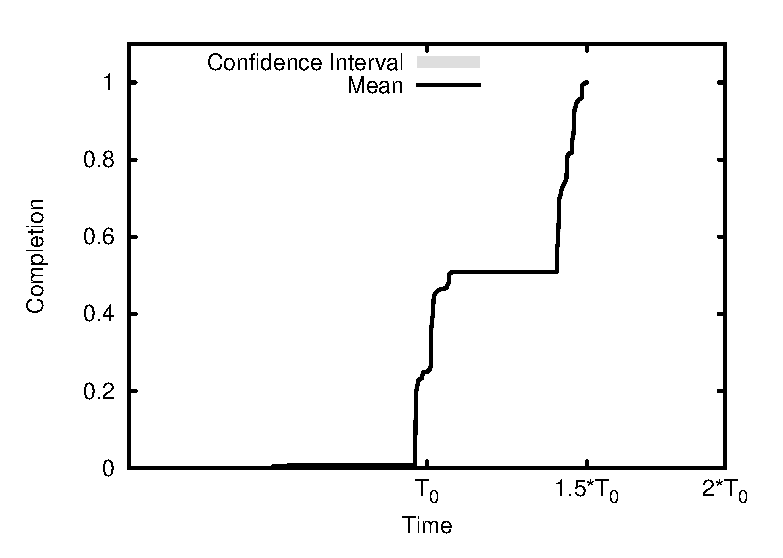
\includegraphics[width=0.49\textwidth]{fig/plots/scenario_1_default/plots/GeneratedMeanChunkCompletion.csv.eps}
    \hfill
    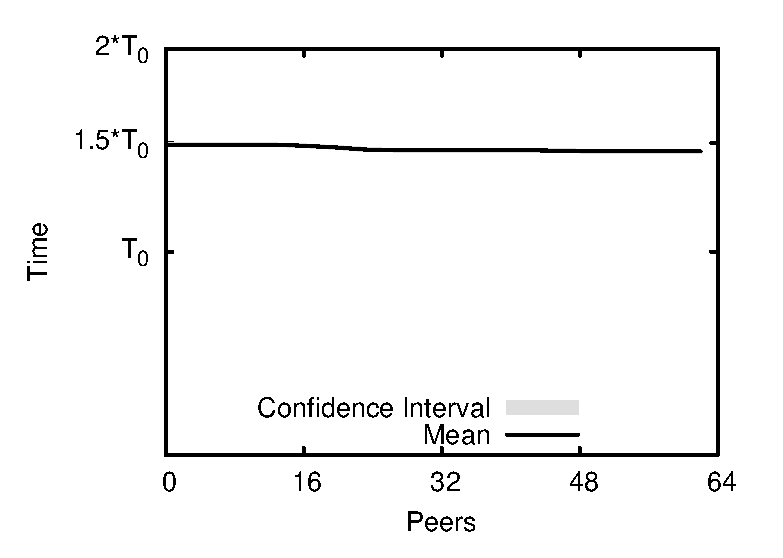
\includegraphics[width=0.49\textwidth]{fig/plots/scenario_1_default/plots/GeneratedMeanSortedChunkCompletion.csv.eps}
  \end{center}
\end{frame}


\begin{frame}
  \frametitle{Default Szenario - Upload/Download}
  \begin{center}
    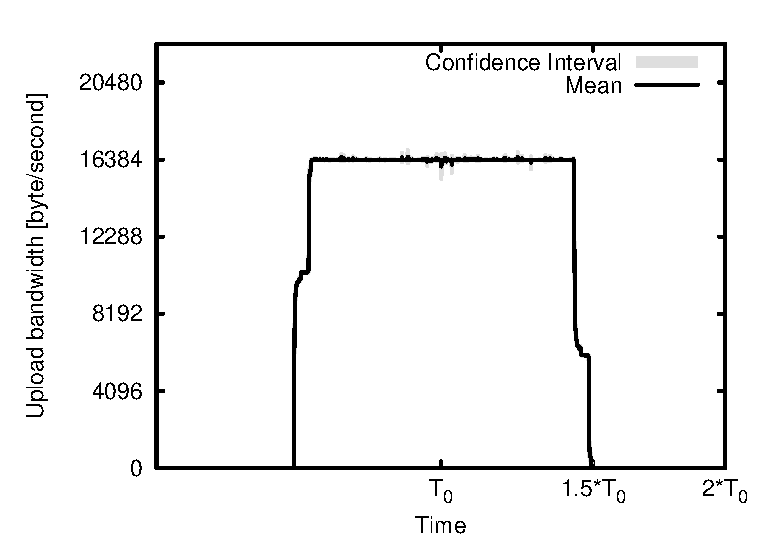
\includegraphics[width=0.49\textwidth]{fig/plots/scenario_1_default/plots/GeneratedMeanCurrentUploadBandwidth.csv.eps}
    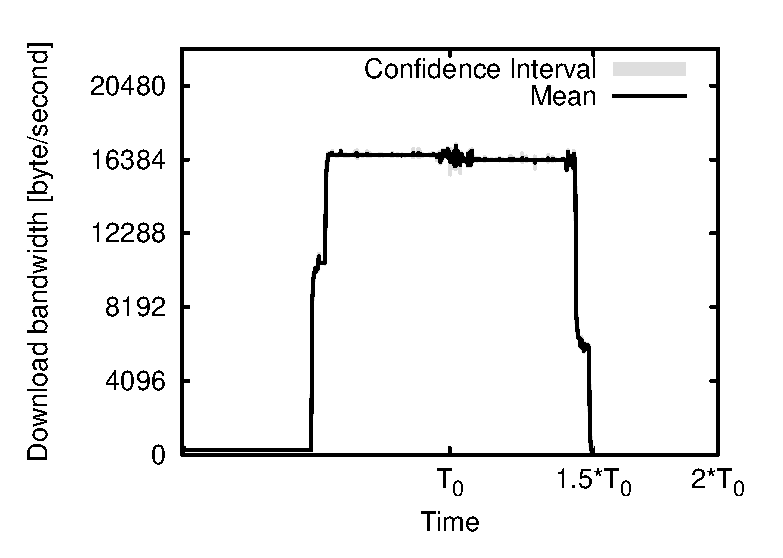
\includegraphics[width=0.49\textwidth]{fig/plots/scenario_1_default/plots/GeneratedMeanCurrentDownloadBandwidth.csv.eps}
  \end{center}
\end{frame}


\begin{frame}
  \frametitle{Default Szenario - Super-Peer Upload}
  \begin{center}
    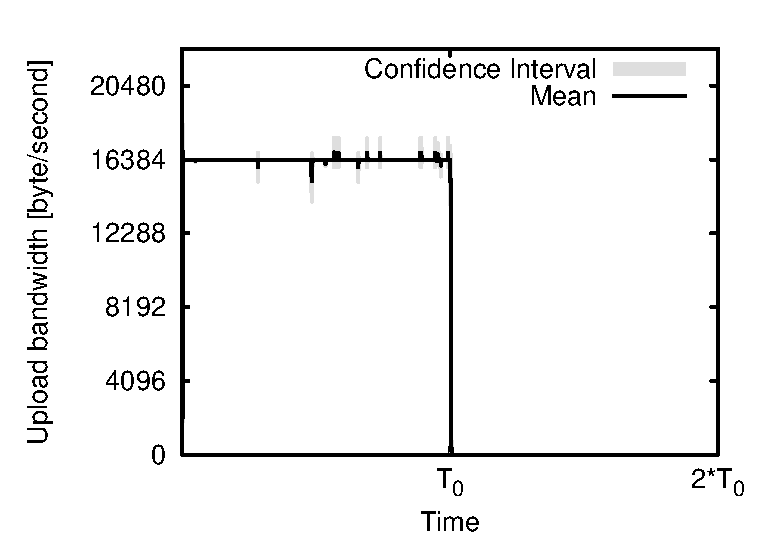
\includegraphics[width=0.49\textwidth]{fig/plots/scenario_1_default/plots/GeneratedMeanCurrentSuperSeederUploadBandwidth.csv.eps}
  \end{center}
\end{frame}

%%%
%%% SCENARIO 128
%%%

\begin{frame}
  \frametitle{Default Szenario mit 128 Peers - Completion}
  \begin{center}
    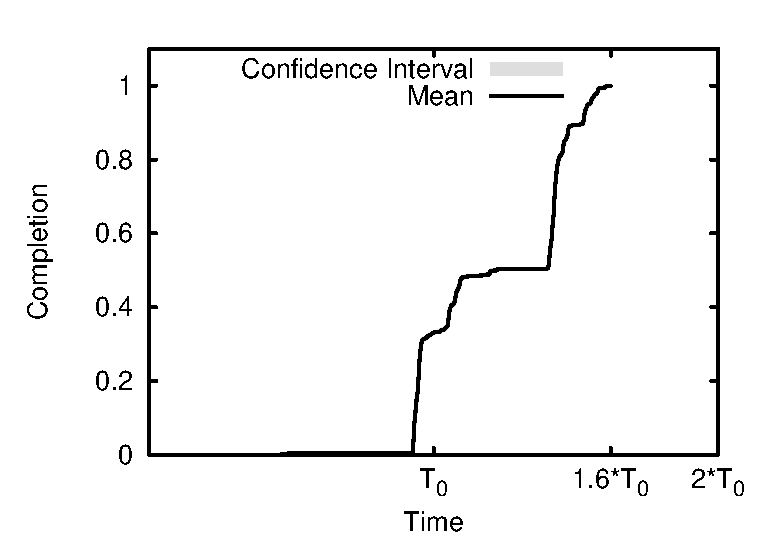
\includegraphics[width=0.49\textwidth]{fig/plots/scenario_4_peer_count_128/plots/GeneratedMeanChunkCompletion.csv.eps}
    \hfill
    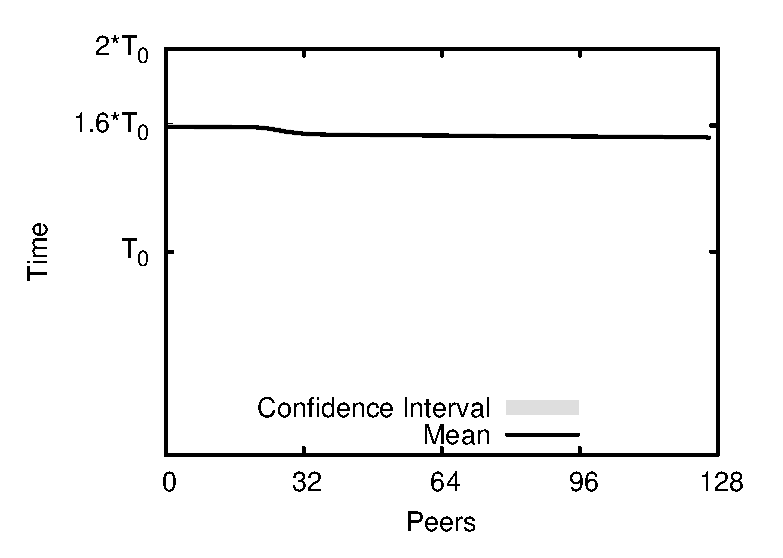
\includegraphics[width=0.49\textwidth]{fig/plots/scenario_4_peer_count_128/plots/GeneratedMeanSortedChunkCompletion.csv.eps}
  \end{center}
\end{frame}


\begin{frame}
  \frametitle{Default Szenario mit 128 Peers - Upload/Download}
  \begin{center}
    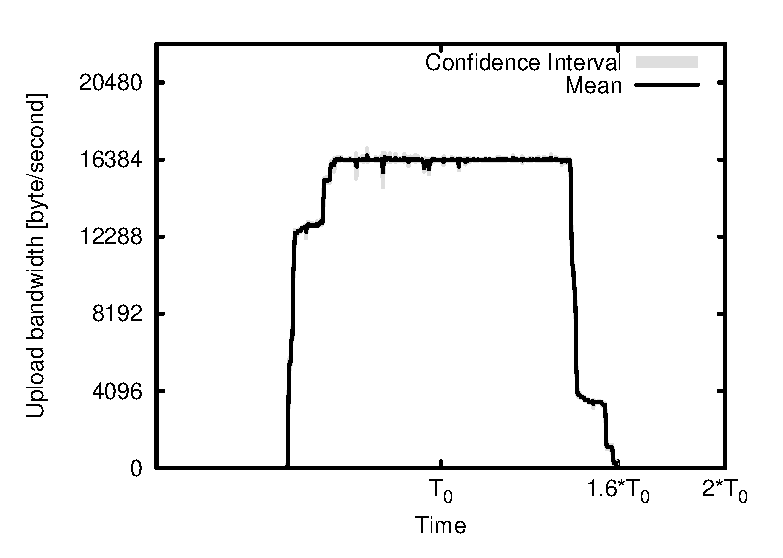
\includegraphics[width=0.49\textwidth]{fig/plots/scenario_4_peer_count_128/plots/GeneratedMeanCurrentUploadBandwidth.csv.eps}
    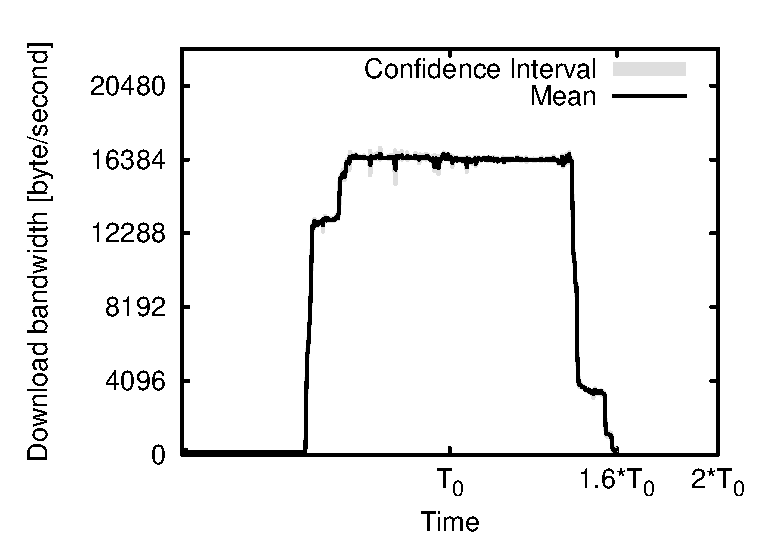
\includegraphics[width=0.49\textwidth]{fig/plots/scenario_4_peer_count_128/plots/GeneratedMeanCurrentDownloadBandwidth.csv.eps}
  \end{center}
\end{frame}


\begin{frame}
  \frametitle{Default Szenario mit 128 Peers - Super-Peer Upload}
  \begin{center}
    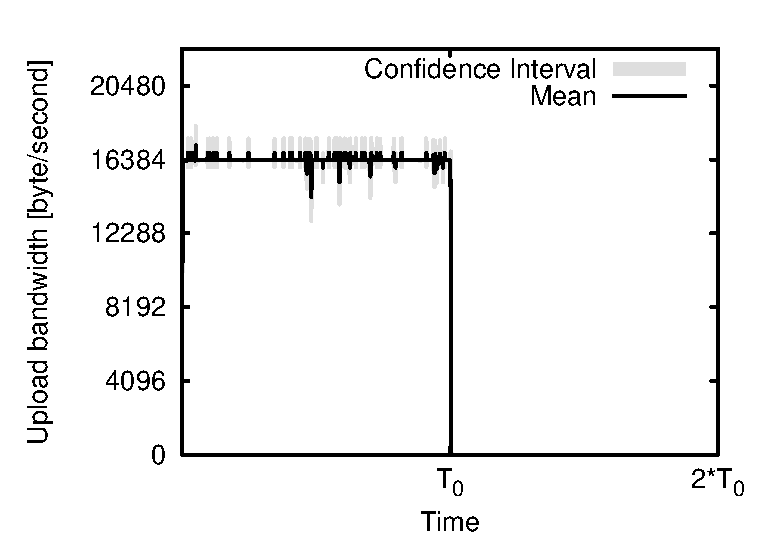
\includegraphics[width=0.49\textwidth]{fig/plots/scenario_4_peer_count_128/plots/GeneratedMeanCurrentSuperSeederUploadBandwidth.csv.eps}
  \end{center}
\end{frame}

%%%
%%% SCENARIO 4x Chunks
%%%

\begin{frame}
  \frametitle{Default Szenario mit 4x Chunkanzahl - Completion}
  \begin{center}
    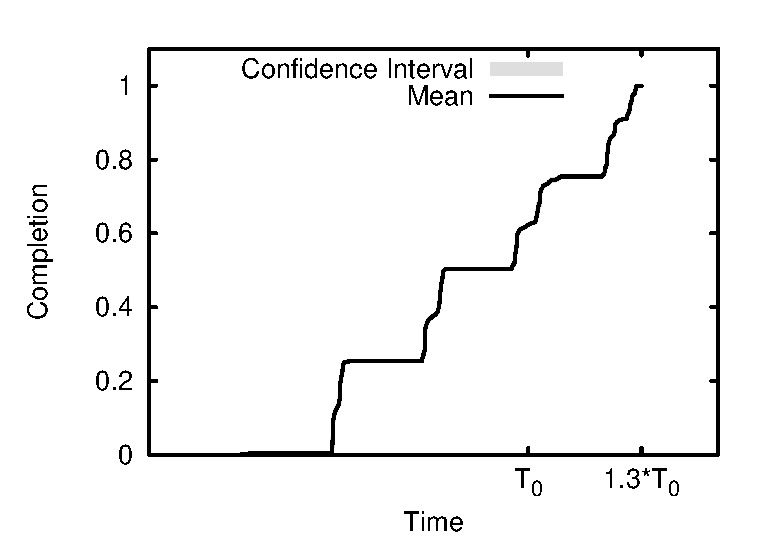
\includegraphics[width=0.49\textwidth]{fig/plots/scenario_15_chunk_count_fac_4/plots/GeneratedMeanChunkCompletion.csv.eps}
    \hfill
    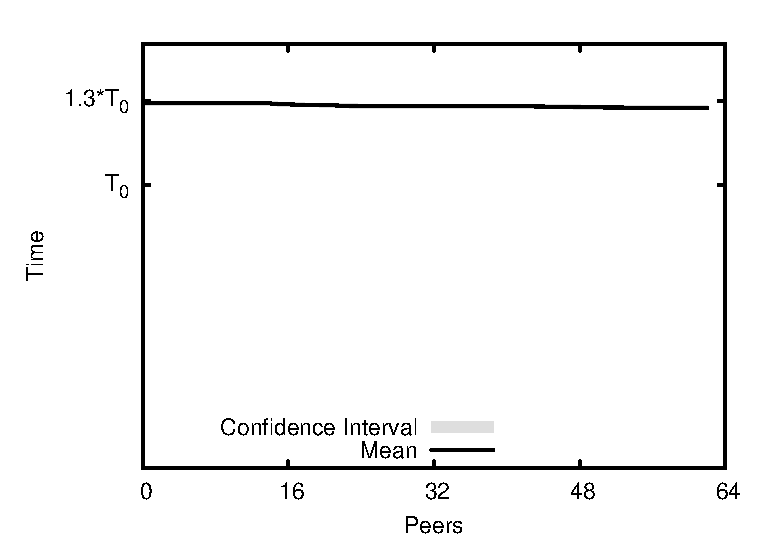
\includegraphics[width=0.49\textwidth]{fig/plots/scenario_15_chunk_count_fac_4/plots/GeneratedMeanSortedChunkCompletion.csv.eps}
  \end{center}
\end{frame}


\begin{frame}
  \frametitle{Default Szenario mit 4x Chunkanzahl - Upload/Download}
  \begin{center}
    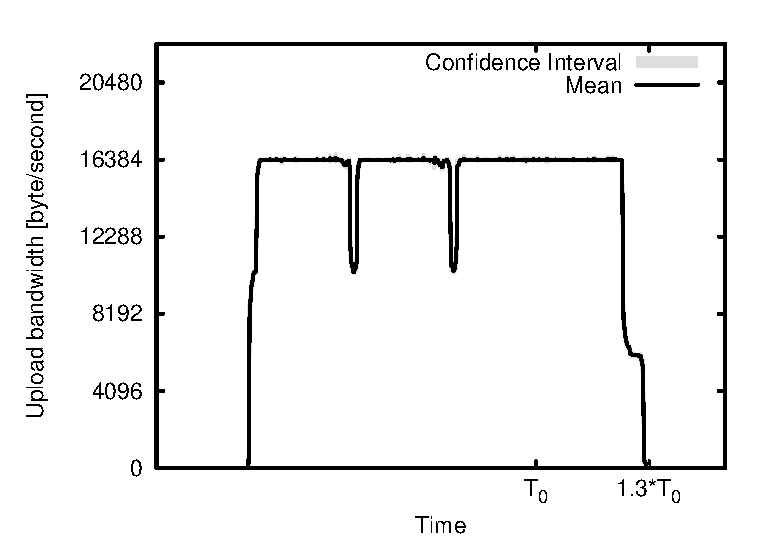
\includegraphics[width=0.49\textwidth]{fig/plots/scenario_15_chunk_count_fac_4/plots/GeneratedMeanCurrentUploadBandwidth.csv.eps}
    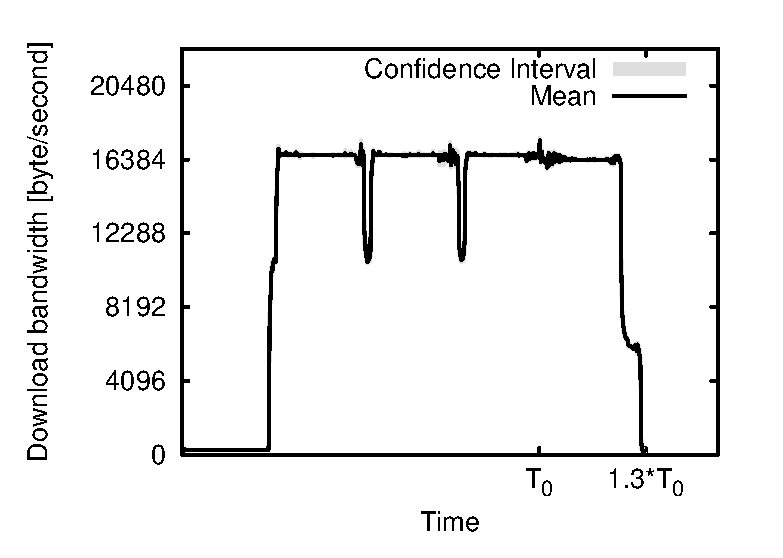
\includegraphics[width=0.49\textwidth]{fig/plots/scenario_15_chunk_count_fac_4/plots/GeneratedMeanCurrentDownloadBandwidth.csv.eps}
  \end{center}
\end{frame}


\begin{frame}
  \frametitle{Default Szenario mit 4x Chunkanzahl - Super-Peer Upload}
  \begin{center}
    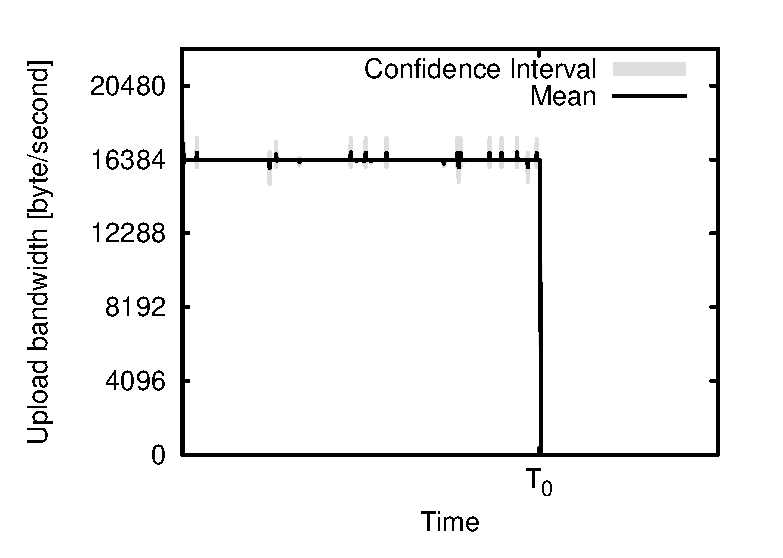
\includegraphics[width=0.49\textwidth]{fig/plots/scenario_15_chunk_count_fac_4/plots/GeneratedMeanCurrentSuperSeederUploadBandwidth.csv.eps}
  \end{center}
\end{frame}


%%%
%%% SCENARIO Parts 20
%%%

\begin{frame}
  \frametitle{Default Szenario mit 20 Datensätzen}
  \begin{block}{Einstellungen}
	  \begin{itemize}  
	    \item Gesamter Datensatz wird in 20 Sub-Datensätze geteilt
	    \vspace{2mm}
	    \item Jeder Sub-Datensatz hat doppelt soviele Chunks wie Peers
	    \vspace{2mm}
	    \item Sub-Datensätze durchnummeriert mit IDs: Kleine IDs zuerst
	    \vspace{2mm}
	    \item Streaming!
	  \end{itemize}		
  \end{block}
\end{frame}

\begin{frame}
  \frametitle{Default Szenario mit 20 Datensätzen - Completion}
  \begin{center}
    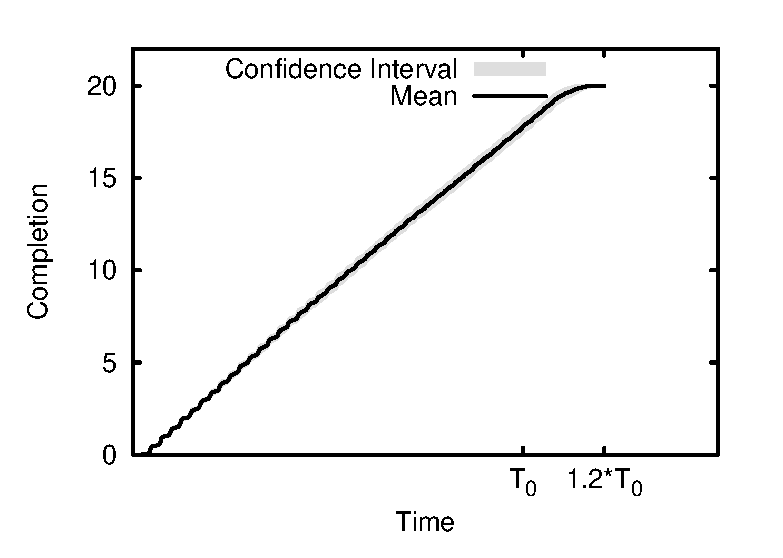
\includegraphics[width=0.49\textwidth]{fig/plots/scenario_6_parts_20/plots/GeneratedMeanChunkCompletion.csv.eps}
    \hfill
    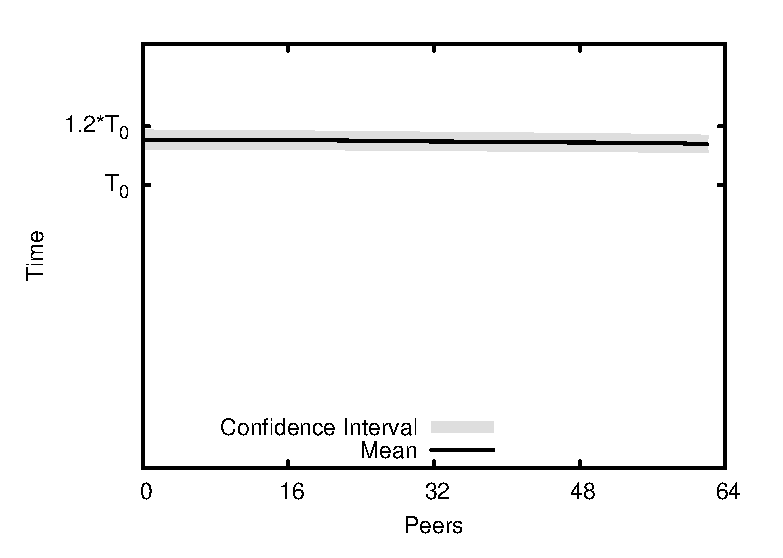
\includegraphics[width=0.49\textwidth]{fig/plots/scenario_6_parts_20/plots/GeneratedMeanSortedChunkCompletion.csv.eps}
  \end{center}
\end{frame}


\begin{frame}
  \frametitle{Default Szenario mit 20 Datensätzen - Upload/Download}
  \begin{center}
    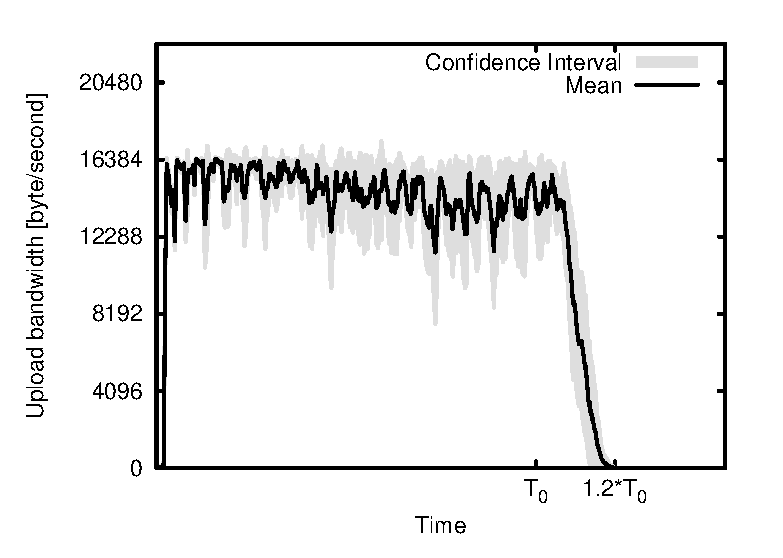
\includegraphics[width=0.49\textwidth]{fig/plots/scenario_6_parts_20/plots/GeneratedMeanCurrentUploadBandwidth.csv.eps}
    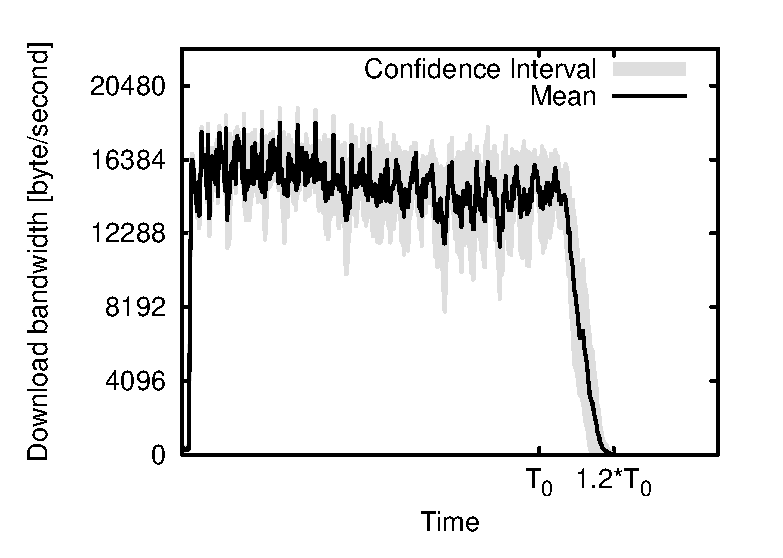
\includegraphics[width=0.49\textwidth]{fig/plots/scenario_6_parts_20/plots/GeneratedMeanCurrentDownloadBandwidth.csv.eps}
  \end{center}
\end{frame}


\begin{frame}
  \frametitle{Default Szenario mit 20 Datensätzen - Super-Peer Upload}
  \begin{center}
    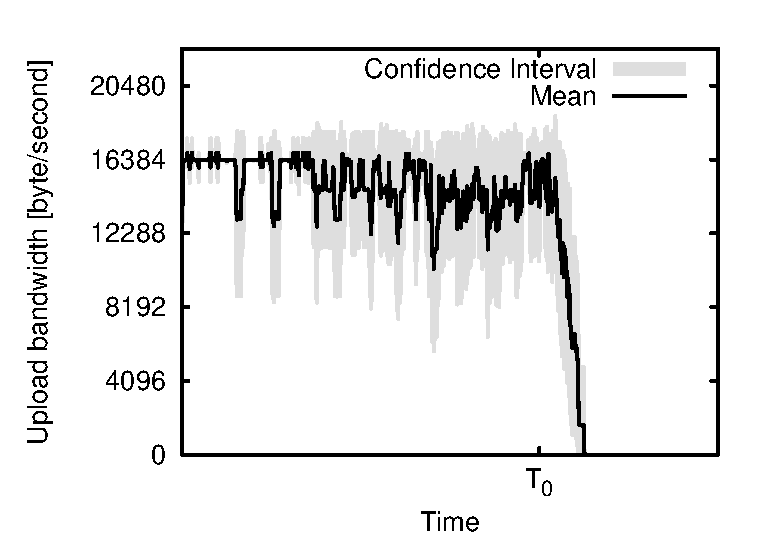
\includegraphics[width=0.49\textwidth]{fig/plots/scenario_6_parts_20/plots/GeneratedMeanCurrentSuperSeederUploadBandwidth.csv.eps}
  \end{center}
\end{frame}



